%%%%%%%%%%%%%%%%%%%%%%%%%%%%%%%%%%%%%%
%%%%%%%%%%%%%%%%%%%%%%%%%%%%%%%%%%%%%%
% Do not edit the TeX file your work
% will be overwritten.  Edit the RnW
% file instead.
%%%%%%%%%%%%%%%%%%%%%%%%%%%%%%%%%%%%%%
%%%%%%%%%%%%%%%%%%%%%%%%%%%%%%%%%%%%%%






Here are results, and a figure. See \fig{example_genes}.
%

\begin{knitrout}
\definecolor{shadecolor}{rgb}{0.969, 0.969, 0.969}\color{fgcolor}\begin{figure}[!h]

{\centering 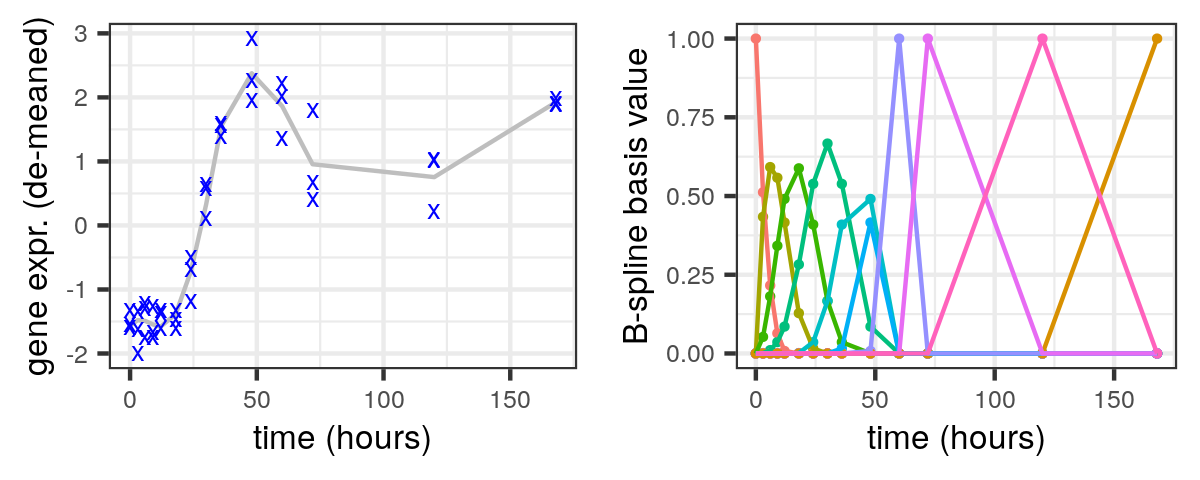
\includegraphics[width=0.98\linewidth,height=0.392\linewidth]{figure/example_genes-1} 

}

\caption[An example gene and regressors]{An example gene and regressors. }\label{fig:example_genes}
\end{figure}


\end{knitrout}
%



\begin{knitrout}
\definecolor{shadecolor}{rgb}{0.969, 0.969, 0.969}\color{fgcolor}\begin{figure}[!h]

{\centering 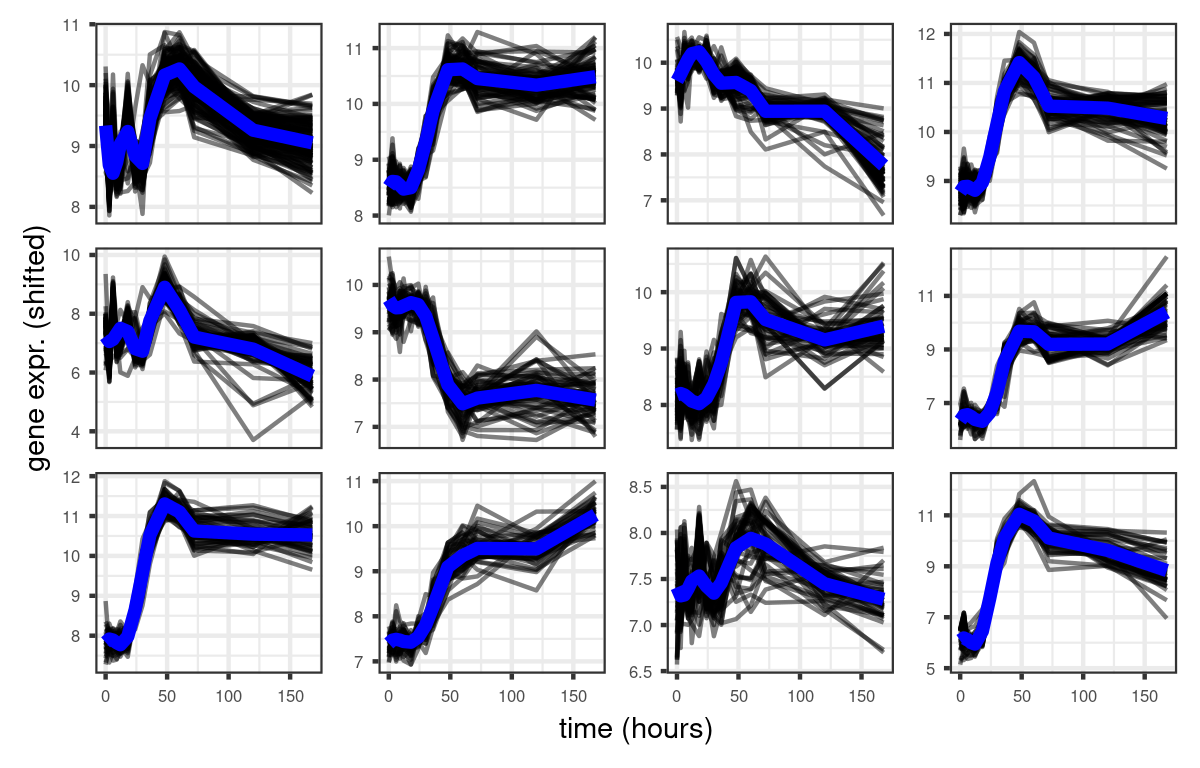
\includegraphics[width=0.98\linewidth,height=0.627\linewidth]{figure/gene_centroids-1} 

}

\caption[Inferred centroids]{Inferred centroids. }\label{fig:gene_centroids}
\end{figure}


\end{knitrout}



\begin{knitrout}
\definecolor{shadecolor}{rgb}{0.969, 0.969, 0.969}\color{fgcolor}\begin{figure}[!h]

{\centering 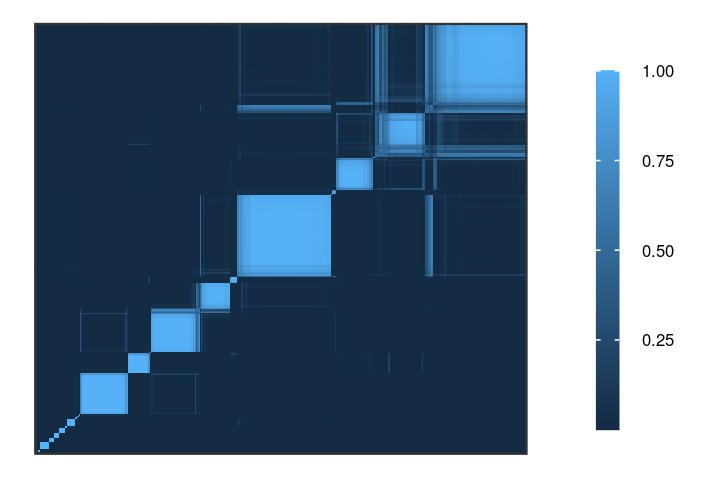
\includegraphics[width=0.98\linewidth,height=0.627\linewidth]{figure/gene_initial_coclustering-1} 

}

\caption[initial co-clustering matrix ]{initial co-clustering matrix }\label{fig:gene_initial_coclustering}
\end{figure}


\end{knitrout}


\begin{knitrout}
\definecolor{shadecolor}{rgb}{0.969, 0.969, 0.969}\color{fgcolor}\begin{figure}[!h]

{\centering 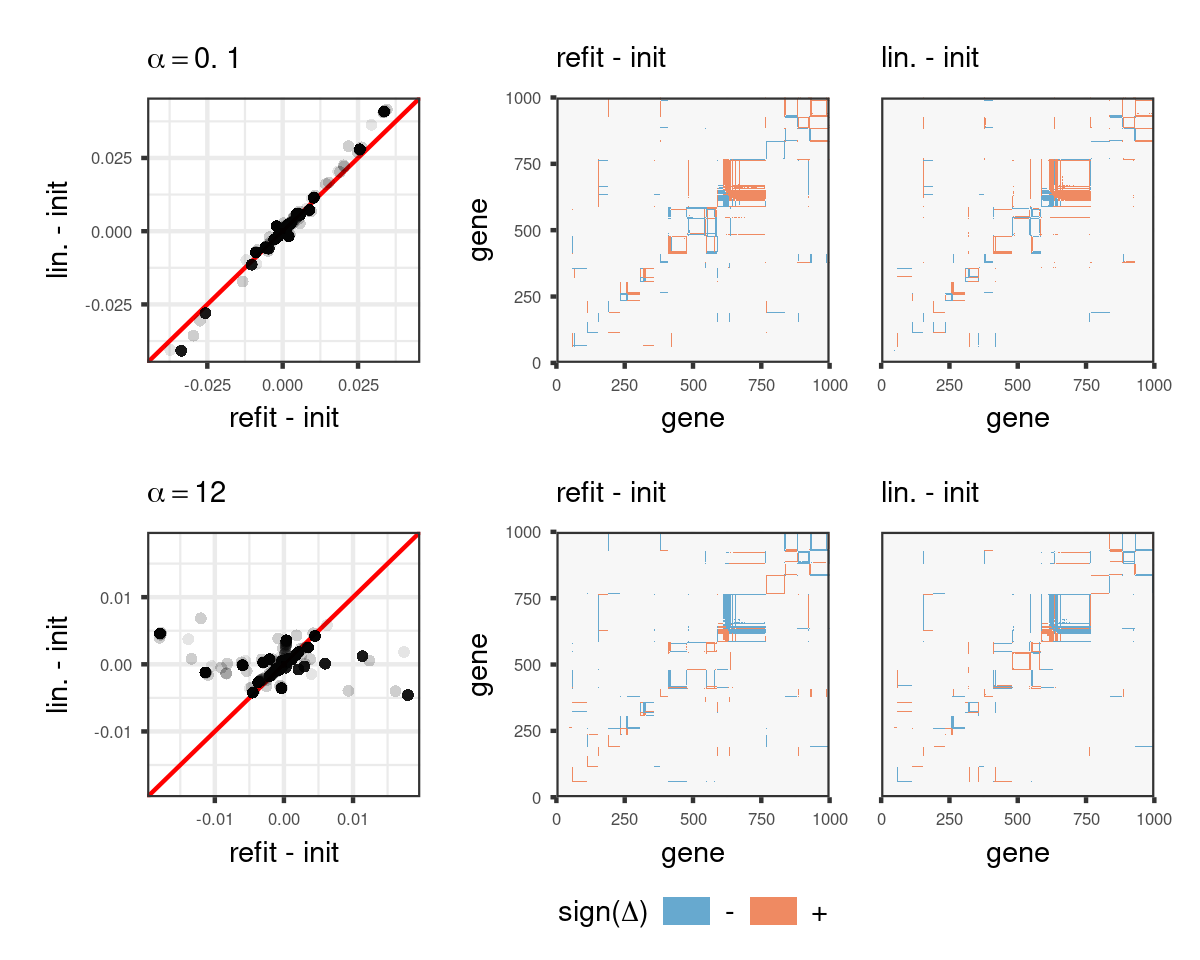
\includegraphics[width=0.98\linewidth,height=0.784\linewidth]{figure/gene_alpha_coclustering-1} 

}

\caption[co-clustering matrix alpha sensitivity]{co-clustering matrix alpha sensitivity}\label{fig:gene_alpha_coclustering}
\end{figure}


\end{knitrout}



\begin{knitrout}
\definecolor{shadecolor}{rgb}{0.969, 0.969, 0.969}\color{fgcolor}\begin{figure}[!h]

{\centering 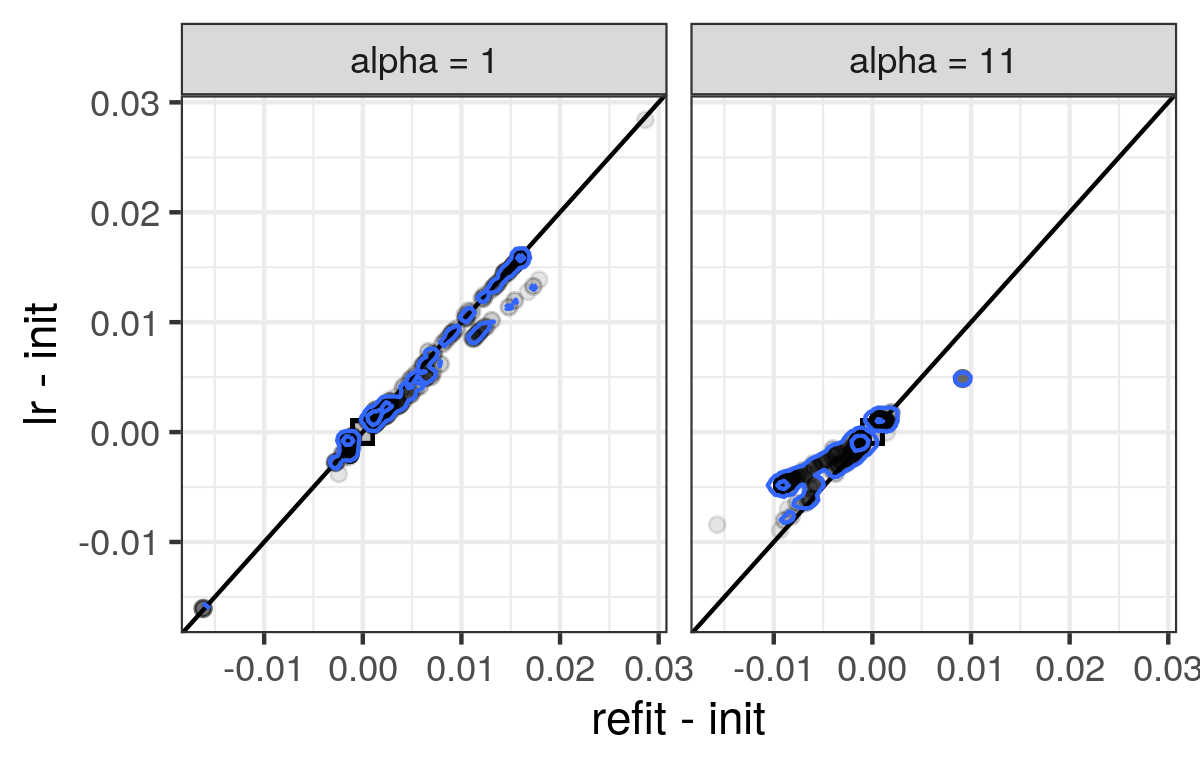
\includegraphics[width=0.98\linewidth,height=0.627\linewidth]{figure/gene_alpha_coclustering_scatter-1} 

}

\caption[co-clustering matrix alpha sensitivity, scatter plot]{co-clustering matrix alpha sensitivity, scatter plot}\label{fig:gene_alpha_coclustering_scatter}
\end{figure}


\end{knitrout}
